\chapter{Introduction}\label{CH:introduction}
Above Earth's atmosphere are the a pair of Van Allen radiation belts, a complex and dynamic plasma environment that effects our technology-driven society. These effects include: a higher radiation dose for astronauts and cosmonauts, higher chance of spacecraft failure due to single event upsets that can lead to catastrophic latchups, degradation of silicon (changing the silicon doping) from an extended radiation dose that can degrade a transistor to the point where it no longer function as a switch, and the degradation of the ozone layer due to the chemical production of $\mathrm{NO_X}$ and $\mathrm{HO_X}$ molecules. With these effects in mind, it is no surprise that the radiation belts have been extensively studied since their discovery in the 1960s.

One natural phenomenon in the radiation belts that has been a topic of interest in the space physics community is wave-particle intersections that, as we will explore throughout this dissertation, can accelerate particles to very high energies (e.g. $\approx \mathrm{MeV}$ for electrons) and scatter them into the atmosphere.

The goal of this dissertation is to study the wave-particle mechanism that scatters microbursts, a sub-second impulse of electrons into Earth's atmosphere. Before we dive deep into the physics of wave-particle interactions, an introduction to Earth's magnetosphere is warranted. Single charged particle motion in Earth's electric and magnetic fields will be described first. Then the major particle populations in the magnetosphere and the coupling between them will be described. Lastly, a brief overview of wave-particle interactions and their effects will be presented.

\section{Charged Particle Motion in Electric and Magnetic Fields}\label{Intro:particle_motion}
A charged particle trapped in the magnetosphere will experience three types of periodic motion in Earth's nearly dipolar magnetic field. The three motions are ultimately due to the Lorentz force that a particle of momentum $\vec{p}$, charge $q$, and velocity $\vec{v}$ experiences in an electric field $\vec{E}$ and magnetic field $\vec{B}$ and is given by
\begin{equation} \label{Intro:Lorentz}
\frac{d\vec{p}}{dt} = q(\vec{E} + \vec{v} \times \vec{B}).
\end{equation} In the magnetosphere, the three periodic motions in decreasing frequency are gyration, bounce, and drift and are schematically shown in Fig. \ref{Intro:motion_diagram}. Each of periodic these motions have a corresponding conserved quantity i.e. an adiabatic invariant. 

\begin{figure}
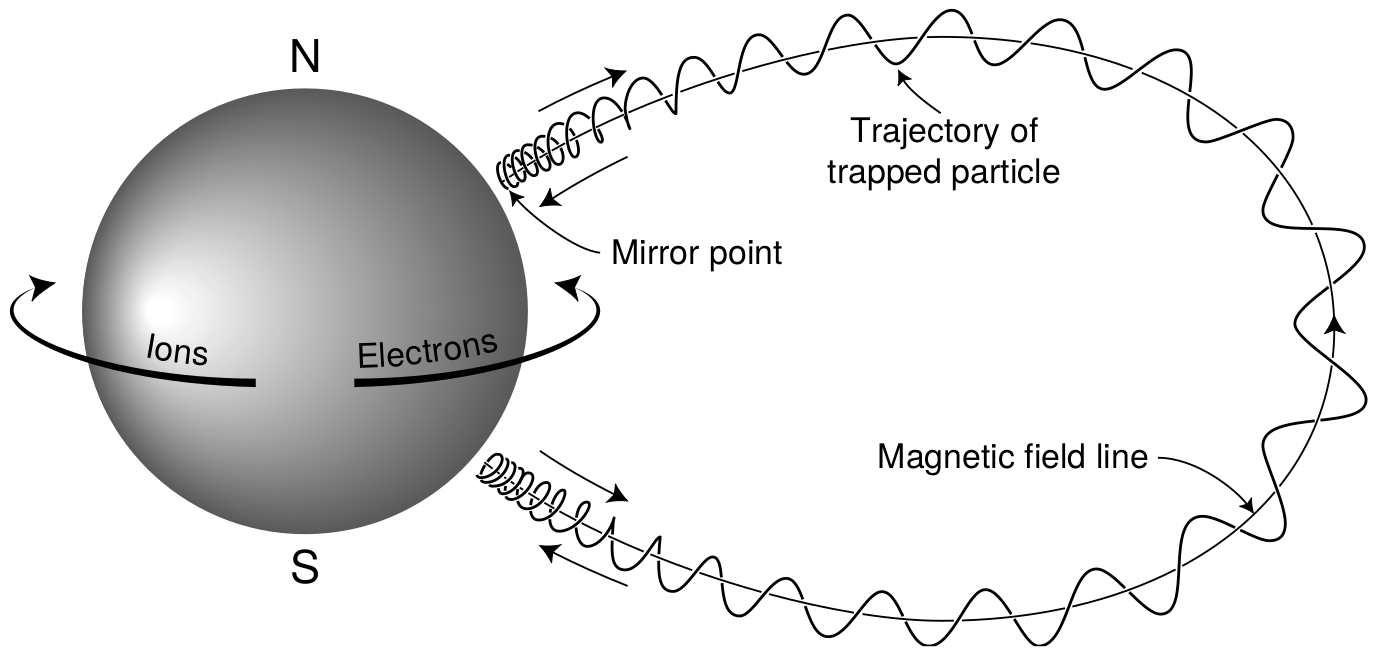
\includegraphics[width=\textwidth]{1_three_motions.png}
\caption{The three periodic motions of charged particles in Earth's dipole magnetic field. These motions are: gyration about the magnetic field line, bounce motion between the magnetic poles, and azimuthal drift around the Earth. Figure from \citep{Baumjohann1997}.}
\label{Intro:motion_diagram}
\end{figure}


The highest frequency periodic motion is gyration about a magnetic field of magnitude $B$. This motion is circular with a Larmor radius of 
\begin{equation}
r = \frac{m v_\perp}{|q| B}
\end{equation} where $m$ is the mass and $v_\perp$ the particle's velocity perpendicular to $\vec{B}$. This motion has a corresponding gyrofrequency 
\begin{equation}
\Omega = \frac{|q| B}{m}
\end{equation} in units of radians/second. Inside the radiation belts the electron gyrofrequency, $\Omega_e$ is on the order of a kHz. The corresponding adiabatic invariant is found by integrating the particle's canonical momentum around the particle's path of gyration
\begin{equation} \label{J}
J_i = \oint (\vec{p} + q \vec{A}) \cdot d\vec{l}
\end{equation} where $J_i$ is the $i^{th}$ adiabatic invariant and $\vec{A}$ is the magnetic vector potential. This integral is carried out by integrating the first term over the circumference of the gyro orbit and integrating the second term using Stokes theorem to calculate the magnetic flux enclosed by the gyro orbit.  With suitable integration, $J_1 \sim v_\perp^2 / B$ and is conserved as the frequency of the driving force, $\omega$ satisfies $\omega << \Omega_e$.

The second highest frequency periodic motion is bouncing due to a parallel gradient in $\vec{B}$. This periodic motion naturally arises in the magnetosphere because Earth's magnetic field is stronger near the poles, and artificially in the laboratory in magnetic bottle machines. To understand this motion we first we need to define the concept of pitch angle $\alpha$ as the angle between $\vec{B}$ and $\vec{v}$ which is schematically shown in Fig. \ref{Intro:pa}a. The pitch angle relates $v$ with $v_\perp$, and $v_{||}$ (the component of the particles velocity parallel to $\vec{B}$). As shown in \ref{Intro:pa}b and c, a larger $\alpha$ will tighten the particle's helical trajectory and vice versa.

Assuming the particle's kinetic energy is concerned, the conservation of $J_1$ implies that given a particle's $v_\perp(0)$ and $B(0)$ at the magnetic equator (where Earth's magnetic field is usually at a minimum), we can calculate its $v_\perp(s)$ along the particle's path $s$ by calculating $B(s)$ from magnetic field models. The particle's perpendicular velocity is then related via
\begin{equation}
\frac{v_\perp^2 (0)}{B(0)} = \frac{v_\perp^2 (s)}{B(s)}
\end{equation} which can be rewritten as 

\begin{equation}
\frac{v^2 \sin^2{\alpha(0)}}{B(0)} = \frac{v^2 - v^2_{||}(s)}{B(s)}
\end{equation} and re-arranged to solve for $v_{||}(s)$

\begin{equation} \label{Intro:eq_vp} 
v_{||}(s) = v \sqrt{1 - \frac{B(s)}{B(0)} \sin^2{\alpha(0)}}
\end{equation} which will tend towards 0 when the second term in the radical approaches 1.

The location where $v_{||}(s) = 0$ is called the mirror point and is where a particle stops and reverses direction. Since Earth's magnetic field is stronger towards the poles, the mirroring particle will execute periodic bounce motion between its two mirror points in the northern and southern hemispheres. The corresponding adiabatic invariant, $J_2$ is

\begin{equation} \label{Intro:j2}
J_2 = \oint p_{||} ds
\end{equation} where $ds$ describes the particle path between the mirror points in the northern and southern hemispheres (see Fig. \ref{Intro:motion_diagram}). $J_2$ is found by substituting Eq. \ref{Intro:eq_vp} into Eq. \ref{Intro:j2} and defining the magnetic field strength at the mirror points as $B_m$ where $\alpha(m) = 90^\circ$. The $J_2$ integral can be written as     
\begin{equation}
J_2 = 2 p \int_{m_n}^{m_s} \sqrt{1 - \frac{B(s)}{B(m)}} ds
\end{equation} where $m_n$ and $m_s$ are the northern and southern mirror points, respectively. The bounce period can be estimated \citep[e.g.][]{Baumjohann1997} to be 

\begin{equation}
t_b \approx \frac{L R_e}{\sqrt{W/m}} (3.7 - 1.6 \sin{\alpha(0)})
\end{equation} where $L$ is the $L$-shell which describes the distance from the Earth's center to the location where a particular magnetic field line crosses the magnetic equator, in units of Earth radii, $R_e$. $W$ is the particle's kinetic energy. As with gyration, a particle bounces as long as $\omega << \Omega_b$, where $\Omega_b$ is the bounce frequency.

At this stage it is instructional to introduce the notion of the loss cone pitch angle, $\alpha_L$.  A particle with $\alpha \leq \alpha_L$ will mirror at or below $\approx 100$ km altitude in the atmosphere. A particle at those altitudes will encounter Earth's atmosphere and has a significant probability of Coulomb scattering with atmospheric particles and be lost to the atmosphere.

\begin{figure}
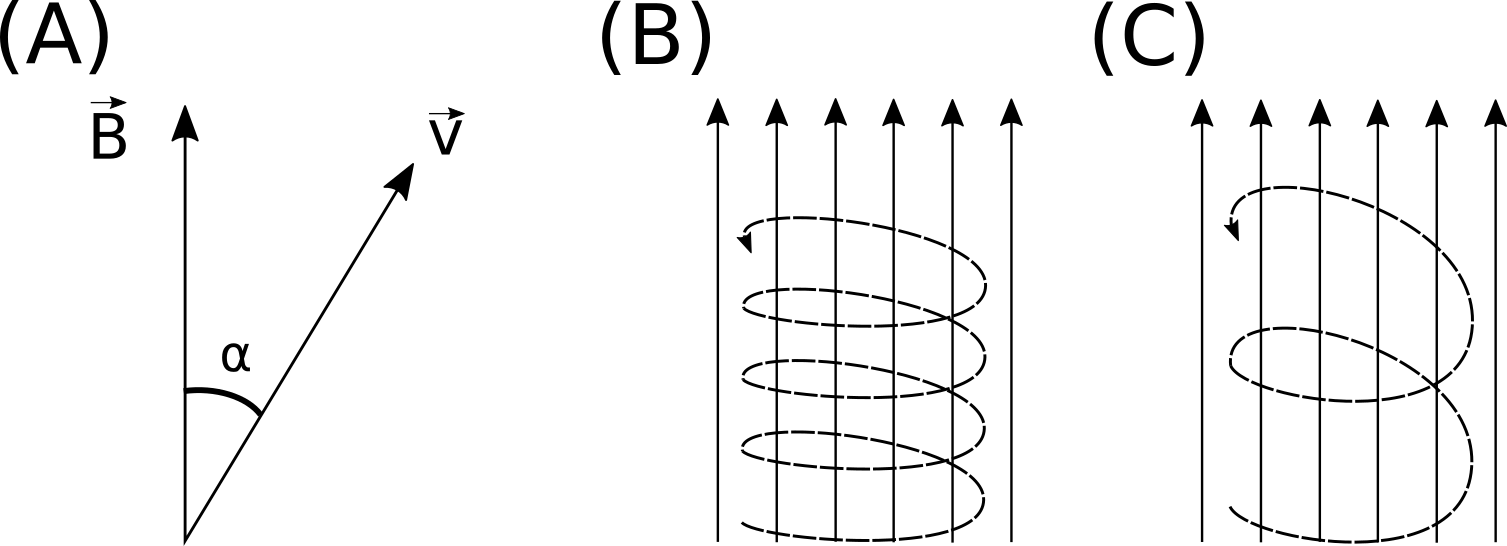
\includegraphics[scale=1]{1_pitch_angle_and_helix.png}
\caption{Charged particle motion in a uniform magnetic field $\vec{B}$. Panel (A) shows the geometry defining the pitch angle, $\alpha$. Panel (B) and (C) show two helical electron trajectories with dashed lines assuming a large and small $\alpha$ (corresponding to a small and large parallel velocity $v_{||}$), respectively.}
\label{Intro:pa}
\end{figure}

The slowest periodic motion experienced by charged particles in Earth's magnetic field is azimuthal drift around the Earth. This drift results from a combination of a radial gradient in $\vec{B}$ and the curvature of the magnetic field. The radial gradient drift arises because Earth's magnetic field is stronger near the Earth where the particle's gyroradius radius of curvature is smaller as it gyrates towards stronger magnetic field, and larger when it gyrates outward. The overall effect is the particle gyro orbit does not close on itself and negatively charged particles drift East and positively charged particles drift West. The radial gradient drift is enhanced by the centrifugal force that a particle experiences as it bounces along the curved field lines. The drift adiabatic invariant, $J_3$ is found by integrating Eq. \ref{J} over the complete particle orbit around the Earth. The shape of this drift orbit is otherwise known as a drift shell. For $J_3$, the first term is negligible and the second term is the magnetic flux enclosed by the drift shell, $\Phi_m$  i.e. $J_3 \sim \Phi_m$. 

Figure \ref{Intro:adiabatic_frequencies} from \citet{Schulz1974} shows contours of the gyration, bounce, and drift frequencies for electrons and protons in Earth's dipole magnetic field. 

\begin{figure}
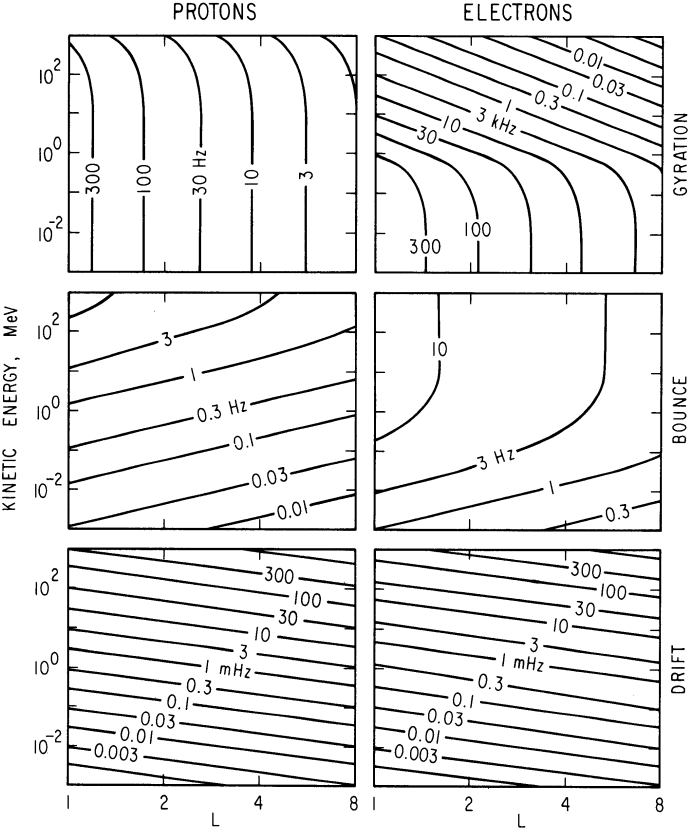
\includegraphics[width=\textwidth]{1_schulz_lanzerotti_fig6.png}
\caption{Contours of constant gyration, bounce, and drift frequencies for electrons and protons in a dipole field. Figure from \citet{Schulz1974}.}
\label{Intro:adiabatic_frequencies}
\end{figure}

Up until now we have considered the three periodic motions due Earth's magnetic field and the absence of electric fields. If $\vec{E}$ is present, a particle's center of gyration i.e., averaged position of the particle over a gyration, will drift with a velocity perpendicular to both $\vec{E}$ and $\vec{B}$. The drift velocity can be solved directly from Eq. \ref{Intro:Lorentz} and is
\begin{equation}
\vec{v}_E = \frac{\vec{E} \times \vec{B}}{B^2}.
\end{equation} Lastly, for more detailed derivations of these motions, see the following texts: \citet{Baumjohann1997, Schulz1974, Tsurutani1997}.
        
\section{Particle Populations and Their Interractions in the Magnetosphere}\label{ntro:particle_populations}
The single-particle motion in Earth's magnetic field described in the previous section is a prerequisite to understanding how magnetospheric  particles organize into macroscopic populations. The structure of the outer magnetosphere is shown in Fig. \ref{Intro:outer_magnetosphere} and inner magnetosphere in Fig. \ref{Intro:inner_magnetosphere}. In this section we will introduce the various particle populations in the magnetosphere and how they couple.

\begin{figure}
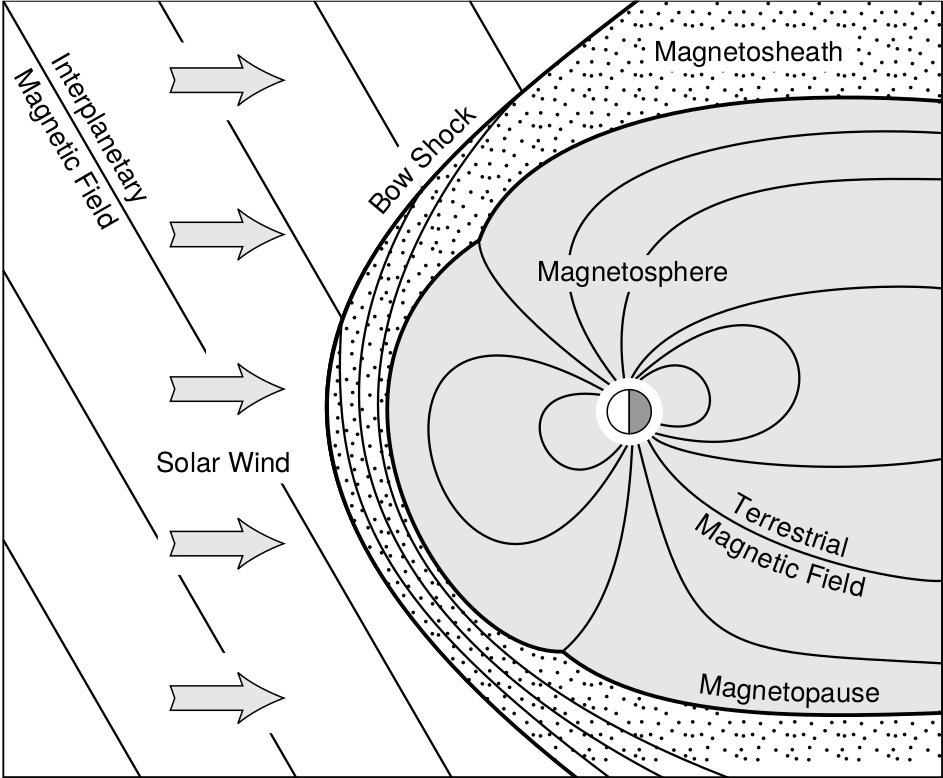
\includegraphics[width=\textwidth]{1_outer_magnetosphere.png}
\caption{Macroscopic structures in the outer magnetosphere. The solar wind with its frozen-in interplanetary magnetic field is shown on the left and is traveling supersonically towards the right. The solar wind envelops Earth's magnetic field to create the magnetosphere cavity. Since the solar wind is traveling supersonically, it creates a bow shock up stream. Downstream of the bow shock the shocked solar wind plasma inside the magnetosheath flows around the magnetopause, a boundary between the solar wind and magnetosphere. Figure from \citet{Baumjohann1997}.}
\label{Intro:outer_magnetosphere}
\end{figure}

\begin{figure}
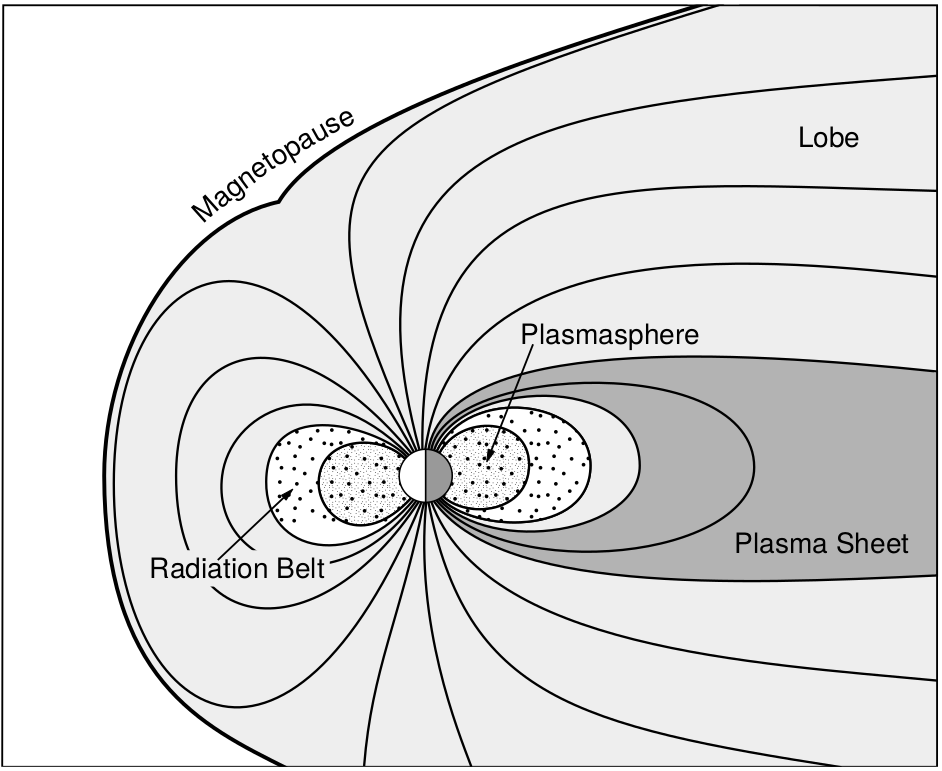
\includegraphics[width=\textwidth]{1_inner_magnetosphere.png}
\caption{Macroscopic structures in the inner magnetosphere most relevant to this dissertation. The plasmasphere, and the radiation belts are shown and ring current is co-located there as well. Sun is to the left. Figure from \citet{Baumjohann1997}.}
\label{Intro:inner_magnetosphere}
\end{figure}

The sun and its solar wind are ultimately the source of energy input into the magnetosphere. The solar wind at Earth's orbit is a plasma traveling at supersonic speeds with an embedded interplanetary magnetic field (IMF). When the solar wind encounters Earth's magnetic field the plasma can not easily penetrate into the magnetosphere, rather it drapes around the magnetosphere forming a cavity in the solar wind that is roughly shaped as shown in Fig. \ref{Intro:outer_magnetosphere}. Because the solar wind is supersonic at 1 AU, a bow shock exists upstream of the magnetosphere. The solar wind plasma, after it is shocked by the bow shock, flows around the magnetosphere inside the magnetosheath. The surface where the solar wind ram pressure and Earth's magnetic pressure balance is termed the magnetopause, which can be thought of as a boundary between the solar wind's and Earth's plasma environments. This is a slightly naive description of the magnetopause, but is nonetheless an instructive conceptual picture. The shocked plasma then flows past the Earth where it shapes the magnetotail. In the magnetotail the solar wind magnetic pressure balances Earth's magnetic field pressure in the lobes. The magnetotail extends on the order of 100 $R_E$ downstream of Earth \textcolor{red}{Add citation}, and the tailward stretching of magnetic field lines creates the plasma sheet which exists in the region of low magnetic field strength near the magnetic equator \textcolor{red}{Add citation}. The plasma sheet flows from dusk to dawn (out of the page in Figs. \ref{Intro:outer_magnetosphere} and \ref{Intro:inner_magnetosphere}) and this current is connected to a zoo of other currents in the magnetosphere which is beyond the scope of this dissertation.

The idea of the magnetopause as a barrier between the solar wind and the magnetosphere is not entirely accurate due to the presence of reconnection. Reconnection was first conceived by \citet{Dungey1961} who described the convection of Earth's magnetic field between the bow and tail regions of the magnetosphere. This process is known as the Dungey cycle and is most effective when the IMF is pointing southward as is shown in Fig. \ref{Intro:reconnection} part 1. As the IMF contacts Earth's magnetic field it reconnects with it so that Earth's magnetic field is directly connected to the IMF. Then as the solar wind flows tailward the IMF drags Earth's magnetic field towards the magnetotail as shown in Fig. \ref{Intro:reconnection} parts 2-6. As more and more magnetic field lines are draped in the magnetotail, magnetic pressure increases in the lobes which squeezes the plasma sheet until Earth's magnetic field reconnects as is shown in Fig. \ref{Intro:reconnection} part 7. Lastly, Fig. \ref{Intro:reconnection} part 8 shows the newly merged magnetic field line and the plasma frozen on it moves Earthward under the magnetic tension force to become more dipolar. This is called a dipolarization of the magnetic field, and the plasma frozen on these field lines can be observed as injections \citep[e.g.][]{Turner2015}. Injection of plasma into the inner magnetosphere is one of the drivers of inner magnetosphere dynamics. \textcolor{red}{Should I talk about the K-H instability and how there could be micro reconnection? i.e. cite a paper or two that support or refute that idea.}

\begin{figure}
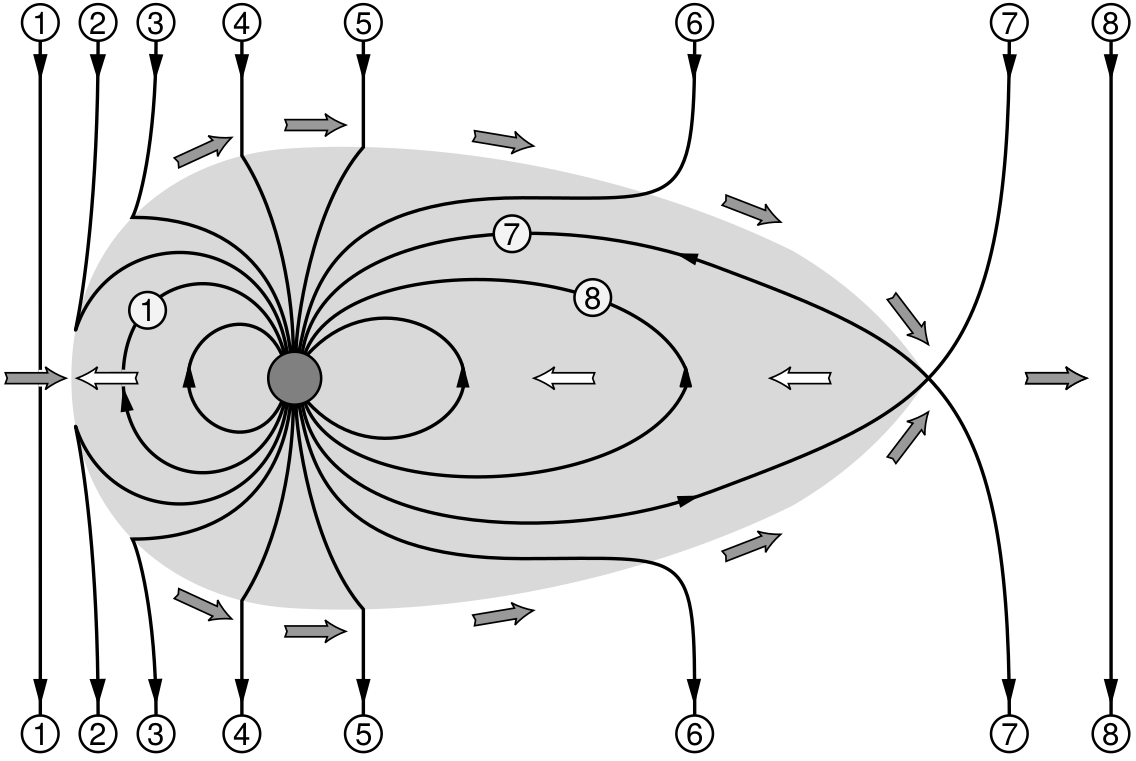
\includegraphics[width=\textwidth]{1_reconnection.png}
\caption{The series of steps involved in magnetic reconnection with a southward IMF. Figure from \citet{Baumjohann1997}.}
\label{Intro:reconnection}
\end{figure}

\subsection{Inner Magnetosphere Populations}\label{Intro:inner_mag}
Before we describe the inner magnetosphere particle populations, we first need to describe the coordinate system used to organize the inner magnetosphere populations. The first coordinate was defined in section \ref{Intro:particle_motion} and is the L shell. L shell can be thought of as an analogue to a radius but in a dipole geometry. The azimuthal coordinate is the magnetic local time (MLT). For an observer above Earth's north pole looking down, MLT is defined to be 0 (midnight) in the anti-sunward direction, and increases in the counter-clockwise direction with 6 at dawn, 12 at noon (sunward direction), and 18 in dusk. The last coordinate used in this dissertation is the magnetic latitude, $\lambda$ which is analogous to the latitude coordinate and is defined to be 0 at the magnetic equator. 

The low energy particle dynamics in the inner magnetosphere are organized by two electric fields: the co-rotation and the dawn-dusk electric fields. The co-rotation electric field arises from the rotation of Earth's magnetic field. Since particles are frozen on magnetic field lines and the plasma conductivity is effectively infinite, to a non-rotating observer, Earth's rotation appears as a radial electric field that drops of as $\sim L^2$. This electric field makes particles orbit around the Earth due to the $\vec{E} \times \vec{B}$ drift. The other electric field, pointing from dawn to dusk is called the convection electric field and is formed by the Earthward transport of particles from the magnetotail that appears as an electric field to a stationary observer (with respect to Earth). The superposition of the co-rotation and and convection electric fields results in a potential field shown in Fig. \ref{Intro:E_fields}. The shaded area in Fig. \ref{Intro:E_fields} shows the orbits on which low energy electrons are trapped, and outside are the untrapped particles. The dynamic topology of the shaded region in Fig. \ref{Intro:E_fields} is controlled by only the convection electric field which is dependent on the solar wind speed and the IMF. The lowest energy particles, that are most effected by these electric fields, make up the plasmasphere.

\begin{figure}
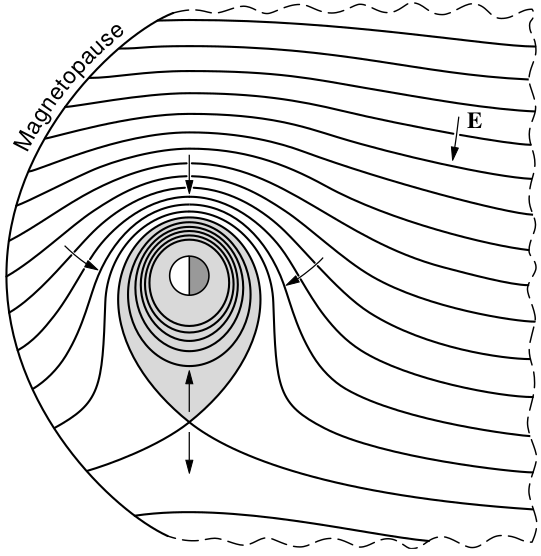
\includegraphics[width=\textwidth]{1_convection_corotation.png}
\caption{Equipotential lines and electric field arrows due to the superposition of the co-rotation and convection electric fields. Electrons in the shaded region execute closed orbits. Outside of the shaded regions the electrons are not trapped and will escape. The region separating the two regimes is called the Alfven layer. Figure from \citet{Baumjohann1997}.}
\label{Intro:E_fields}
\end{figure}

\subsubsection{Plasmasphere}
The plasmasphere is a dense ($n_e \sim 10^3/\mathrm{cm}^3$), cool plasma ($\sim \mathrm{eV}$) that extends to $L \sim 4$ (extent is highly dependent on the solar wind and magnetospheric conditions) and is sourced from the ionosphere. The two main mechanisms that source the cold plasma from the ionosphere are ultraviolet ionization by sunlight and particle precipitation. The ultraviolet ionization by sunlight is strongly dependent on the time of day (day vs night), latitude (more ionization near the equator). The ionization due to particle precipitation, on the other hand, is highly dependent on magnetospheric conditions, and mostly occurs at high latitudes.

The outer boundary of the plasmasphere is the plasmapause which is typically identified as a steep radial gradient in plasma density from $\sim 10^3 / \mathrm{cm}^3$ to $\sim 1 / \mathrm{cm}^3$. As we will see throughout this dissertation, the location of the plasmapause is important to model \citep[e.g.][]{O'Brien2003empirical} and understand since the plasma density strongly controls the efficiency of particle scattering \citep{Horne2005}.

\subsubsection{Ring Current}
The next higher energy population is the ring current. This population consists of protons and electrons between tens and a few hundred keV that drift around the Earth. The orbits of higher energy particles are not as effected by the convection and co-rotation electric field, rather they drift around the Earth due to gradient and curvature drifts. Since the direction of the drift is dependent on charge, protons drift west around the Earth and electrons drift East. This has the effect of creating a current around the Earth. 

The ring current generates a magnetic field which decreases the magnetic field strength on Earth's surface and increases it outside of the ring current. The decrease of Earth's magnetic field strength is readily observed by a system of ground-based magnetometers and is merged into a Disturbance Storm Time (DST) index. An example of a DST index time series from a coronal mass ejection (CME) driven 2015 St. Patrick's Day storm is shown in Fig. \ref{Intro:dst}. The ring current is sometimes first depleted and DST increases slightly (initial phase or sudden storm commencement). Then the ring current is rapidly built up during which DST rapidly decreases (main phase). Lastly the ring current gradually decays toward its equilibrium state over a period of a few days and DST increases towards 0 (recovery phase). The DST index along with other indicies are readily used by the space physics community to quantify the global state of the magnetosphere.

\begin{figure}
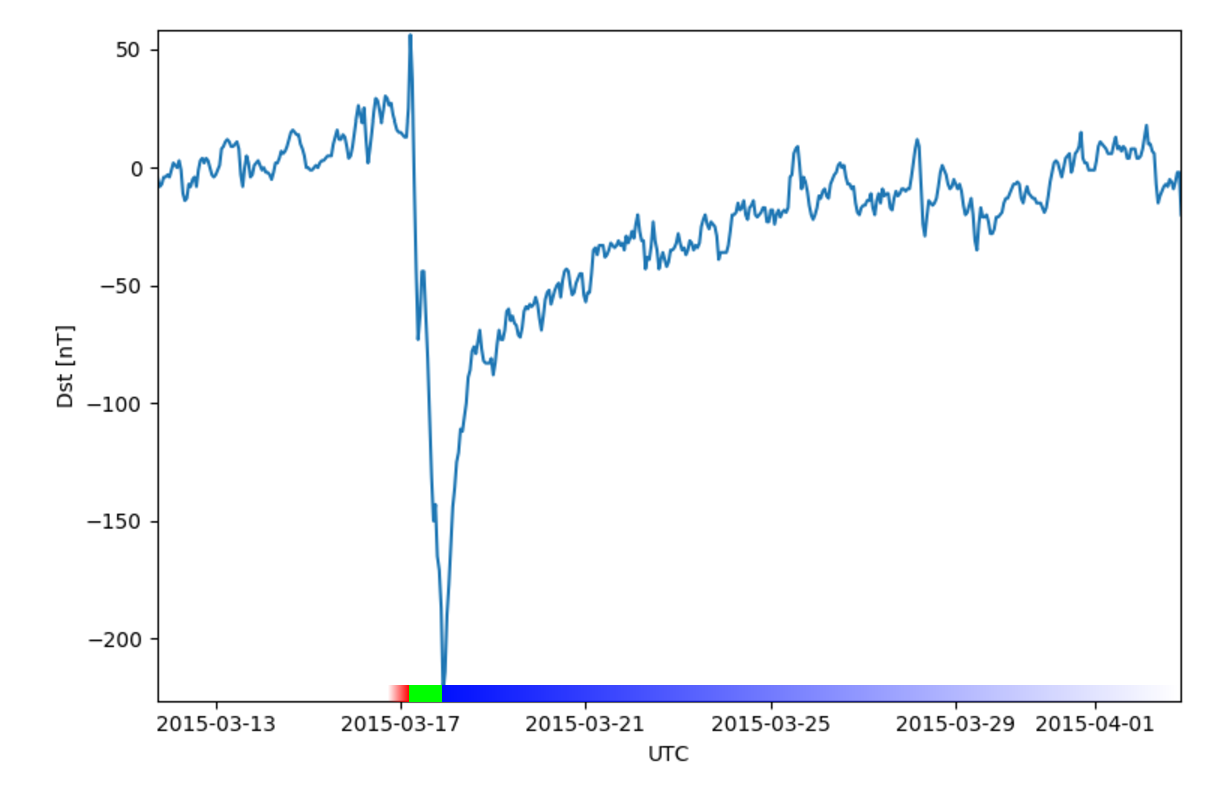
\includegraphics[width=\textwidth]{1_dst.pdf}
\caption{The DST index during the St. Patrick's Day 2015 storm. This storm was caused by a coronal mass ejection on March 15th, 2015. The storm phases are: initial phase, main phase, and recovery phase. The initial phase occurred when the Dst peaked at +50 nT on March 17th during which the ring current was eroded by the coronal mass ejection during the interval shown by the red bar. Then the rapid decrease to $\approx -200$ nT was during the main phase where many injections from the magnetotail pumped up the ring current which reduced Earth's magnetic field strength at the ground and is shown with the green bar. Lastly, the recovery phase lasted from March 18th to approximately March 29th during which the ring current particles were lost and the ring current returned to its equilibrium state. The recovery phase is shown with the blue bar.}
\label{Intro:dst}
\end{figure}

\subsubsection{Radiation Belts}\label{Intro:radiation_belt}
The highest energy particle populations are in the Van Allen radiation belts. These belts were discovered by \citet{Allen1959} and \citet{Vernov1960} during the Cold War and are a pair of toroidally shaped populations of trapped electrons and protons usually within to $L < 8$ and are shown in Fig. \ref{Intro:rad_belts}. Their quiescent toroidal shape is similar to the shape of the plasmasphere and ring current and is a result of Earth's dipole magnetic field and the conservation of the three adiabatic invariants discussed in section \ref{Intro:particle_motion}.

\begin{figure}
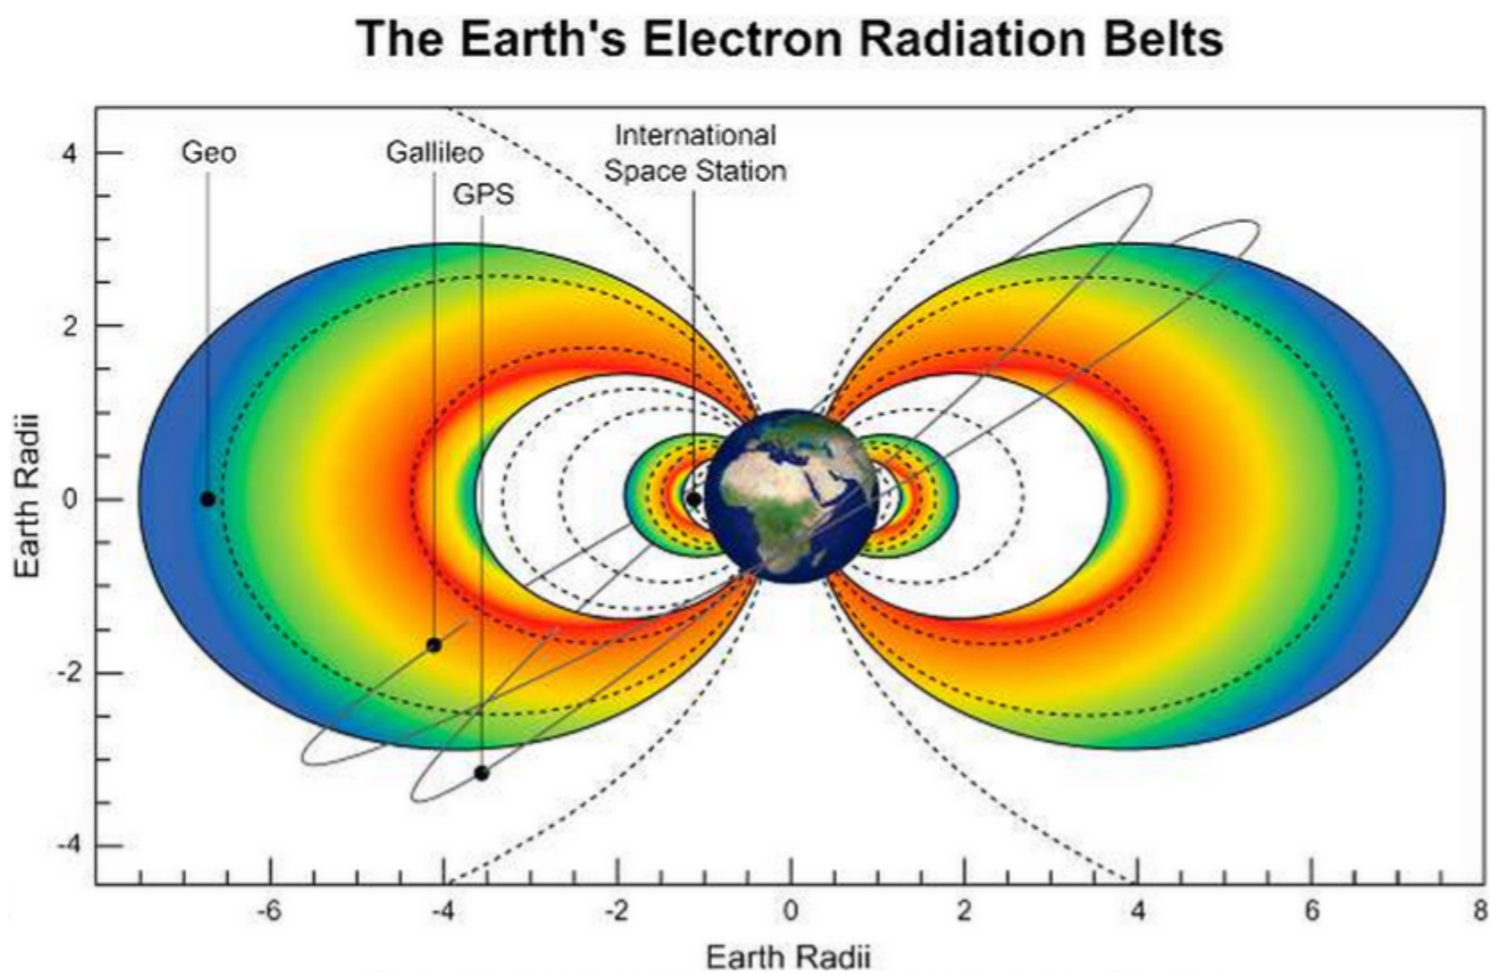
\includegraphics[width=\textwidth]{1_rad_belt.png}
\caption{The two radiation belts with a the locations of various satelites and orbits. Figure from \citep{Horne2013}.}
\label{Intro:rad_belts}
\end{figure}

\begin{figure}
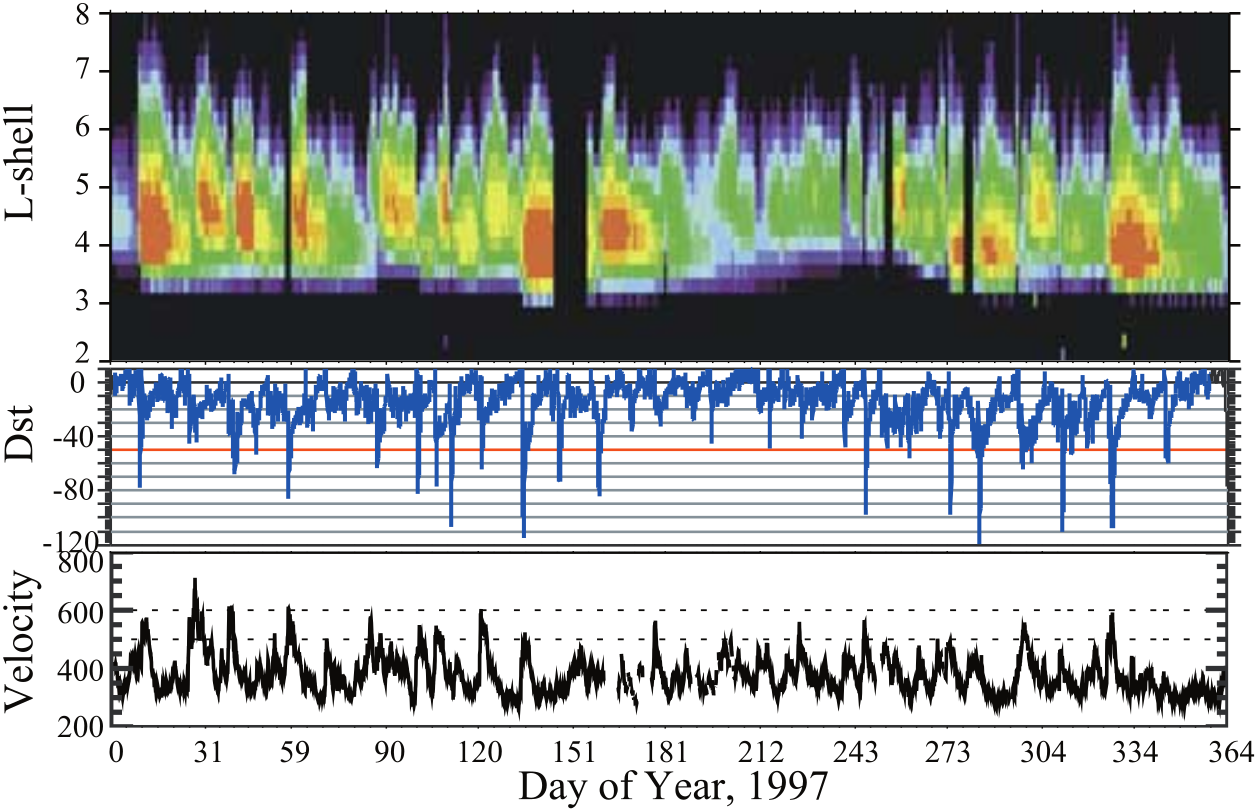
\includegraphics[width=\textwidth]{1_reeves_l_cut.png}
\caption{The dynamics of the outer radiation belt in 1997 from the POLAR satellite. Top panel shows the 1.2-2.4 MeV electron flux as a function of L and 1997 day of year. The middle panel shows the DST index, and bottom panel shows the solar wind velocity. Figure from \citep{Reeves2003}.}
\label{Intro:reeves_l_cut}
\end{figure}

The inner radiation belt is extremely stable on time periods of years, extends to $L \approx 2$, and mainly consists of protons with energies between MeV and GeV and electrons with energies up to $\approx 1$ MeV \citep{Claudepierre2019}. The source of inner radiation belt protons is believed to be due to cosmic-ray albedo neutron decay \citep[e.g.][]{Li2017_CRAND} and inward radial diffusion for electrons \citep[e.g.][]{O'Brien2016_inner}. The gap between the inner and outer radiation belt is called the slot, which is believed to be due to hiss waves inside the plasmasphere (described below) scattering particles into the atmosphere \citep[e.g.][]{Lyons1973, Breneman2015}.

The outer radiation belt, on the other hand is much more dynamic and consists of mainly electrons of energies up to a few MeV. The outer belt's spatial extent is highly variable e.g. see Fig. \ref{Intro:reeves_l_cut}, and is typically observed at $4 < L < 8$. Since the outer radiation belt contains a dynamic population of energetic particles that pose a threat to human and technological presence in Earth's atmosphere and space, decades of research has been undertaken to understand and predict the outer radiation belt particles, waves, and wave-particle interactions. The dynamics of the outer radiation belt can be understood by considering various competing acceleration and loss mechanisms which will be described in the following sections.

\section{Radiation Belt Particle Sources and Sinks}\label{Intro:sources_sinks}

\subsection{Adiabatic Heating}\label{Intro:adiabatic_heating}
One of the particle heating and transport mechanisms arises from the Earthward convection of particles. The conservation of $J_1$ implies that the initial and final $v_\perp$ depends on the change in the magnetic field amplitude

\begin{equation}
\frac{v^2_{\perp \ i}}{B_i} = \frac{v^2_{\perp \ f}}{B_f}.
\end{equation} As a particle convents Earthward, $B_f > B_i$ thus $v_\perp$ must increase. The dipole magnetic field amplitude can be written as

\begin{equation}
B(L, \theta) = \frac{31.2 \ \mathrm{\mu T}}{L^3}\sqrt{1 + 3 \cos^2 \theta}
\end{equation} which implies that 

\begin{equation}
\frac{v_{\perp \ f}^2}{v_{\perp \ i}^2} = \bigg( \frac{L_i}{L_f} \bigg)^3.
\end{equation}.

In addition, as the particle convects Earthward the distance between the particle's mirror points decrease. If $J_2$ is conserved, the shrinking bounce path implies that $v_{||}$ must increase by 

\begin{equation}
\frac{v_{|| \ f}^2}{v_{|| \ i}^2} = \bigg( \frac{L_i}{L_f} \bigg)^k
\end{equation} where $k$ ranges from $2$ for equatorial pitch angles, $\alpha_{eq} = 0^\circ$, to $2.5$ for $\alpha_{eq} = 90^\circ$ \citep{Baumjohann1997}. Since the rate of adiabatic heating is greater in the perpendicular direction than heating in the parallel direction, an initially isotropic particle distribution will become anisotropic during its convection. These isotropic particles can then become unstable to wave growth and generate waves in order to reach equilibrium.


\subsection{Wave Resonance Heating}\label{Intro:wave_heating}
Another mechanism that heats particles is due to particles resonating with plasma waves. A few of the electromagnetic wave modes responsible for particle acceleration (and deceleration) relevant to radiation belt dynamics are hiss, whistler mode chorus (chorus), and electromagnetic ion cyclotron (EMIC) waves. These waves are created by the loss cone instability that driven by an anisotropy of electrons for chorus waves, and protons for EMIC waves. The level of anisotropy can be quantified by the ratio of the perpendicular to parallel particle temperatures $(T_\perp/T_{||})$. A particle distribution is unstable when $T_\perp/T_{||} > 1$ which facilitates wave growth. Since electrons gyrate in a right-handed sense, the chorus waves also tend to be right hand circularly polarized \citep{Tsurutani1997}. The same argument applies to protons and left hand circularly polarized EMIC waves as well. 

These circularly polarized waves can resonate with electrons and/or protons when their combined motion results in a static $\vec{E}$. One example of a resonance between a right hand circularly polarized wave and an electron is shown in Fig. \ref{Intro:resonance} and is termed the cyclotron resonance. An electron's $v_{||}$ and the wave's parallel wave vector, $k_{||}$ are in opposite directions such that the wave frequency $\omega$ is Doppler shifted to an integer multiple of the $\Omega_e$ at which point the electron feels a static electric field and is accelerated or decelerated. This acceleration happens when a resonance condition is satisfied between a wave and a particle for which we will now derive an illustrative toy model.

\begin{figure}
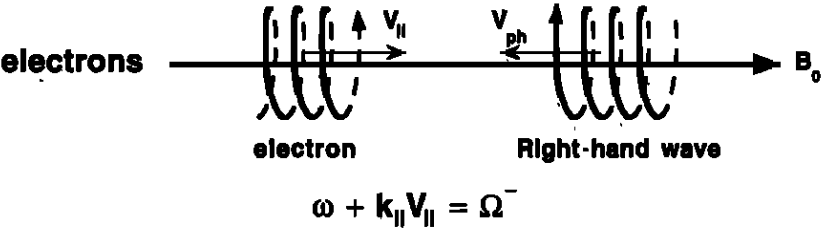
\includegraphics[width=\textwidth]{1_resonance.png}
\caption{The trajectories of an electron and a right-hand circularly polarized wave during a cyclotron resonance. The electron's $v_{||}$ and the wave's $k_{||}$ are in opposite directions such that the wave's frequency is Doppler shifted to a integer multiple of the electron cyclotron frequency. Figure from \citep{Tsurutani1997}.}
\label{Intro:resonance}
\end{figure}

Assume a uniform magnetic field $\vec{B} = B_0 \hat{z}$ with a parallel propagating ($k = k\hat{z}$), right-hand circularly polarized wave. The wave's electric field as a function of position and time can be written as

\begin{equation}
\vec{E} = E_0 (\cos{(\omega t - kz)}\hat{x} + \sin{(\omega t - kz)}\hat{y}) 
\end{equation} which is more clearly expressed by taking the dot product to find $\vec{E}$ in the $\hat{\theta}$ direction
\begin{equation}
E_\theta = \vec{E} \times \hat{\theta} = E_0 \cos{(\omega t - kz + \theta)}.
\end{equation} Now assume that the electron is traveling in the $-\hat{z}$ direction with a velocity $\vec{v} = -v_0 \hat{z}$ so its time dependent position along $\hat{z}$ is

\begin{equation}
z(t) = -v_0 t
\end{equation} and gyrophase is

\begin{equation}
\theta(t) = -\Omega t + \theta(0)
\end{equation} where the first negative sign comes from the electron's negative charge. Now we put this all together and express the electric field and the force that the electron will experience

\begin{equation}
m \frac{dv_\theta}{dt} = qE_\theta = qE_0 \sin{((\omega + kv_0 - \Omega)t + \theta(0))}.
\end{equation} This is a relatively complex expression, but when the time dependent component, 

\begin{equation} \label{Intro:resonance}
\omega + kv_0 - \Omega = 0,
\end{equation} the electron will be in a static electric field which will accelerate or decelerate the electron depending on $\theta_0$, the phase between the wave and the electron. \textcolor{red}{Show Bortnik 2008 plot?} The expression in Eq. \ref{Intro:resonance} is commonly referred to as the resonance condition and is more generally written as 

\begin{equation}
\omega - k_{||} v_{||} = \frac{n \Omega_e}{\gamma}
\end{equation} where $n$ is the resonance order, and $\gamma$ is the relativistic correction \citep[e.g.][]{Millan2007}. It is important to remember that along the particle's orbit it will encounter and experience the effects of all of the waves along its orbit. The typical MLT extent of a handful of waves that are capable of scattering radiation belt electrons are shown in Fig. \ref{Intro:waves}.

\begin{figure}
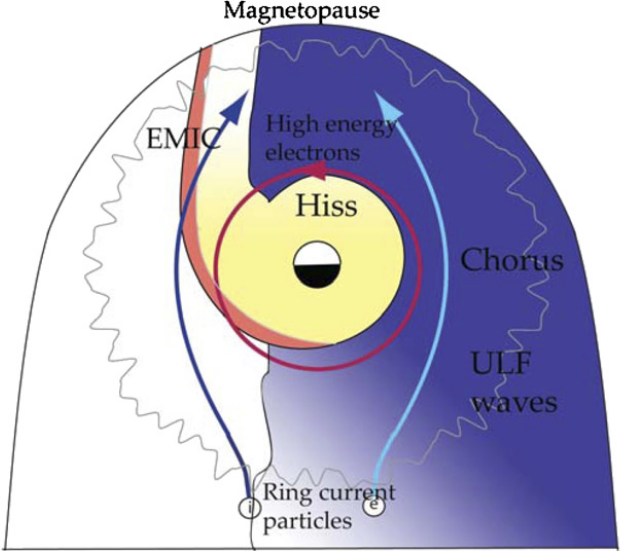
\includegraphics[width=\textwidth]{1_wave_populations.png}
\caption{Various wave modes in the magnetosphere. Ultra low frequency waves occur throught the magnetosphere. Chorus waves are typically observed in the 0-12 midnight-dawn region. EMIC waves are typically observed in the dusk MLT sector. Hiss waves are observed inside the plasmasphere. Figure from \citet{Millan2007}.}
\label{Intro:waves}
\end{figure}

\subsection{Particle Losses}\label{Intro:losses}
There are various transport or scatter mechanisms that result in the loss of radiation belt particles into the atmosphere or the solar wind. One of the loss mechanisms of particles into the solar wind is magnetopause shadowing \citep{Ukhorskiy2006}. Recall that when the ring current is strengthened, the magnetic field is reduced on Earth's surface and increased outside of the ring current. If the time scale of the ring current strengthening is slower than a particle drift, the third adiabatic invariant is conserved. In order to conserve the third adiabatic invariant while the magnetic field strength is increasing outside of the ring current, the particle's orbit gradually moves outward. If the particle drift shell crosses the magnetopause the particle will then be lost to the solar wind.

\textcolor{red}{Move to acceleration?}
Another particle loss (and acceleration) mechanism is driven by ultra low frequency (ULF) waves and is called radial diffusion. Radial diffusion is the transport of particles from high to low phase space density, $f$. If the transport is radially inward, particles will appear to be accelerated. On the other hand, radially outward radial diffusion can transport particles through the magnetopause where they will be lost. \citet{Reeves2013} investigated the driver of particle acceleration during the October 2012 storm and observationally found that inward radial diffusion was not dominant, rather local acceleration via pitch angle diffusion which will be described bellow appeared to be the dominant acceleration mechanism.

The loss mechanism central to this dissertation is pitch angle and energy scattering of electrons by waves such as plasmaspheric hiss \citep[e.g.][]{Breneman2015}, EMIC waves \citep[e.g.][]{Capannolo2019energetic}, and chorus waves \citep[e.g.][]{Breneman2017}. These wave-particle interactions occur when the resonance condition in Eq. \ref{Intro:resonance} is satisfied. When it is satisfied the particle's energy and $\alpha$ is modified by the wave. If the wave changes $\alpha$ towards $0$ such that $\alpha < \alpha_{LC}$, the particle's mirror point lowers below $\approx 100$ km altitude and can be lost due collisions with air. Some of these electrons can be impulsively scattered into the loss cone where they are observed as a sub second duration enhancements termed microbursts.

%\subsubsection{Electromagnetic Ion Cyclotron Wave Driven}\label{Intro:emic_scattering}

%\subsubsection{Whistler Mode Chorus Wave Driven}\label{Intro:chorus_scattering}

\section{Microbursts}\label{Intro:microbursts}
\citet{Anderson1964} first reported microbursts from high altitude balloon observations of bremsstrahlung X-rays emitted by microburst electrons impacting the atmosphere. Over the decades since then, microbursts have been observed on many other balloon missions \citep[e.g.][]{Anderson2017, Parks1967, Woodger2015}. In addition to the X-ray signature, microbursts electrons have been directly observed in LEO with LEO spacecraft including the Solar Anomalous and Magnetospheric Particle Explorer (SAMPEX), Focused Investigation of Relativistic Electron Bursts: Intensity, Range, and Dynamics II (FIREBIRD-II), Science Technologies Satellite (STSAT-I)  \citep[e.g.][]{Blake1996, Blum2015, Lorentzen2001a, Lorentzen2001b, Nakamura1995, Nakamura2000, O'Brien2003, O'Brien2004, Crew2016, Breneman2017, Lee2005, Lee2012}. An example microburst time series is shown in Fig. \ref{Intro:microbursts}.

\begin{figure}
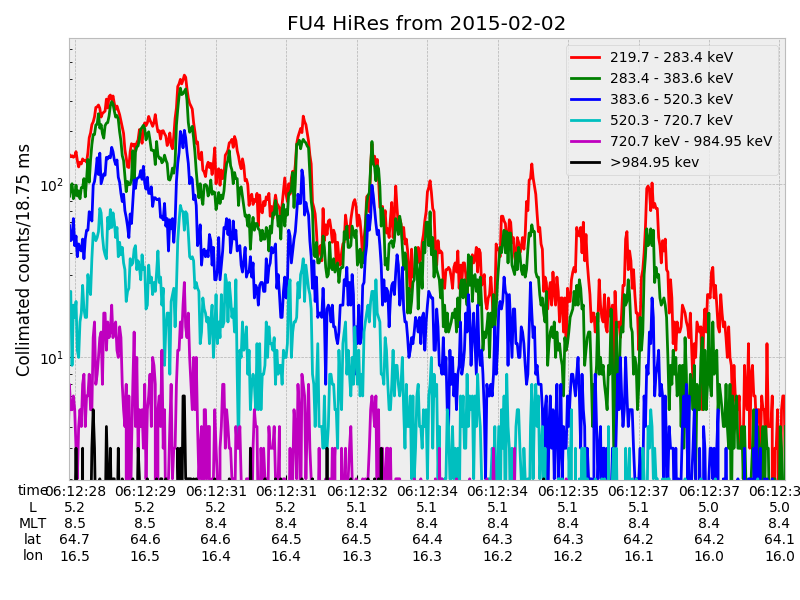
\includegraphics[width=\textwidth]{1_microbursts.png}
\caption{An example train of microbursts observed by FIREBIRD-II unit 4 on February 2nd, 2015. The colored curves show the differential energy channel count rates in six channels from $\approx 200$ keV to greater than 1 MeV. The x-axis labels show auxiliary information such as time of observation and the spacecraft position in L, MLT, latitude and longitude coordinates.}
\label{Intro:microbursts}
\end{figure}

\begin{figure}
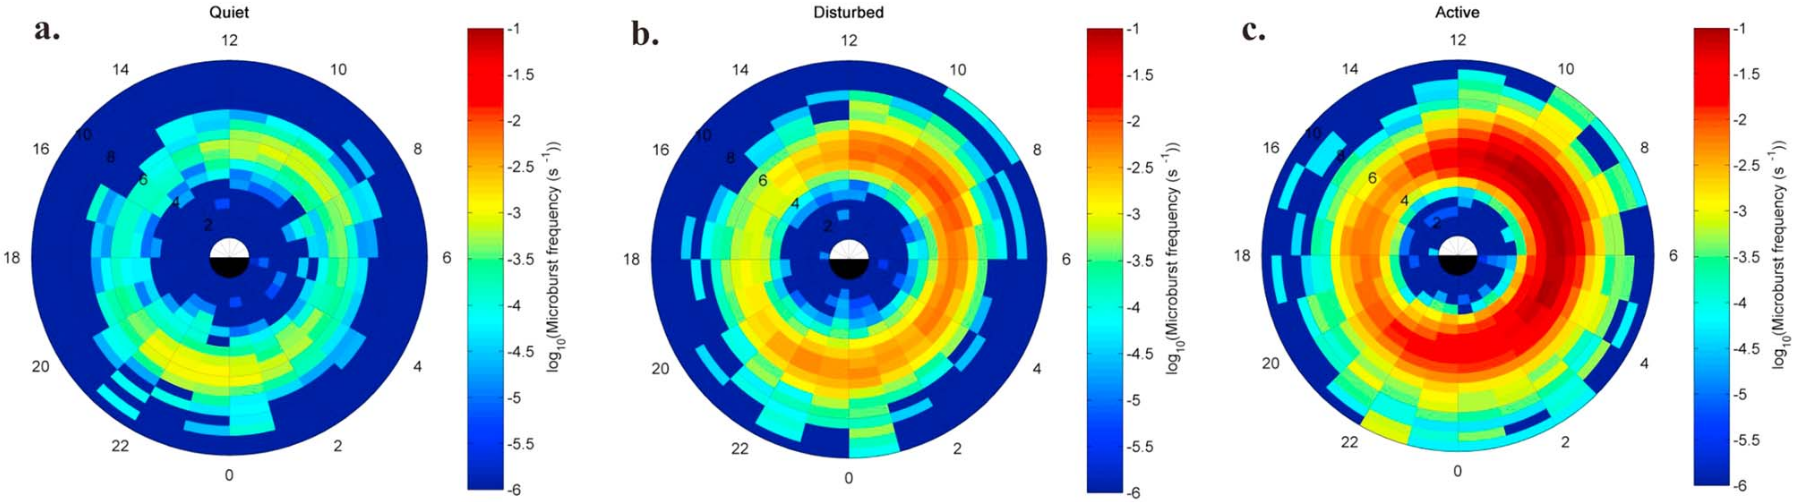
\includegraphics[width=\textwidth]{1_microburst_distribution_douma.png}
\caption{Relativistic $(> 1 \mathrm{MeV})$ distribution of microburst occurrence rates as a function of L and MLT. The three panels explore the microburst occurrence rate dependence on geomagnetic activity parameterized by the auroral electrojet index for (a) $\mathrm{AE} < 100$ nT, (b) $100 < \mathrm{AE} < 300$ nT and (c) $\mathrm{AE} > 300$ nT. Figure from \citet{Douma2017}.}
\label{Intro:microburst_distribution}
\end{figure}

Microbursts are observed on magnetic field footprints that are connected to the outer radiation belt, and are predominately observed in the 0-12 MLT sector with an elevated occurrence frequency during disturbed times as shown in Fig. \ref{Intro:microburst_distribution}. Microbursts have been observed over a wide energy range from a few tens of keV \citep{Datta1997} to greater than 1 MeV \citep[e.g.][]{Blake1996, Greeley2019}. The microburst electron flux ($J$) vs energy spectra is typically well fit to a decaying exponential (e.g. \citep{Parks1967, Lee2005})

\begin{equation}
J(E) = J_0 e^{-E/E_0}
\end{equation} where $J_0$ is the flux at 0 keV (unphysical free parameter) and $E_0$ quantifies the efficiency of the scattering mechanism in energy. A small $E_0$ suggests that mostly high energy particles are scattered and a high $E_0$ suggests that the scattering mechanism scatters low and high energy electrons. In reality, a high $E_0$ may be a signature of a high energy electron scattering mechanism, but is hidden by the convolution of the source particles available to be scattered (typically with a falling energy spectrum) and the energy-dependent scattering efficiency.

The short microburst duration observed by a single LEO satellite creates an ambiguity in interpreting what is exactly a microbursts. Is a microburst very small and spatially stationary so that the LEO spacecraft flies through it in less than a second, or are microbursts large, but short duration such that the microburst comes and goes in a fraction of a second? A high altitude balloon provides essentially a stationary view of the radiation belt footprints and a temporal microburst can be unambiguously identified, but a spatial structure is very difficult to identify.

Multi-spacecraft missions are better equipped to determine if a microburst is spatial or temporal. As will be shown in this dissertation, if a microburst is observed simultaneously by two spacecraft then it is temporally transient with a size greater than the spacecraft separation. On the other hand, if two spacecraft observe a microburst-like feature in the same location and at different times, then it is spatial and called a curtain \citep{Blake2016}.

the microburst size and if it is spatial or temporal, and a balloon can easily observe the temporal microbursts but have limited spatial information. Both observation methods have a unique set of strengths and weaknesses, and this dissertation takes the multi-spacecraft approach to analyze the size of microbursts.


\section{Scope of Reserach}\label{Intro:scope}
This dissertation furthers our understanding of the microburst scattering mechanism and is organized into the following chapters. Chapter \textcolor{red}{X} will describe the spacecraft missions used to study microburst precipitation and wave-particle scattering. Then Ch. \textcolor{red}{Y} will describe a microburst scattering event observed by NASA's Van Allen Probes and the quasi-linear diffusion model that was developed. Next, Ch. \textcolor{red}{Z} will describe a bouncing packet microburst observation made by MSU's FIREBIRD-II mission where the microburst's lower bound longitudinal and latitudinal scale sizes were estimated. Chapter \textcolor{red}{ZZ} then expands the case study result from Ch. \textcolor{red}{Z} to a statistical study of microburst sizes and the microburst size models developed to interpret the data. Lastly, \textcolor{red}{ZZZ} will summarize the dissertation work and make concluding remarks about research to be done.

\textcolor{red}{Mention a theme for the three papers.}